\documentclass[DM,authoryear,toc]{lsstdoc}
% lsstdoc documentation: https://lsst-texmf.lsst.io/lsstdoc.html
\input{meta}

% Package imports go here.
\usepackage{xspace}
\usepackage{hyperref}


% Local commands go here.
\newcommand{\es}{Early Science\xspace}
\newcommand{\dpdd}{Data Products Definition Document (DPDD)\xspace}
\newcommand{\dpv}{Data Preview\,}\xspace
\newcommand{\dpvs}{Data Previews\,}\xspace
\newcommand{\dpzero}{Data Preview 0 (DP0)\,}\xspace
\newcommand{\dpone}{Data Preview 1 (DP1)\,}\xspace
\newcommand{\dptwo}{Data Preview 2 (DP2)\,}\xspace
\newcommand{\drone}{Data Release 1 (DR1)\,}\xspace
\newcommand{\tvssc}{Transients and Variable Stars Science Collaboration (TVSSC)\xspace}
\newcommand{\sssc}{Solar System Science Collaboration (SSSC)\xspace}
\newcommand{\diffim}{Difference Imaging\,}\xspace
\newcommand{\drp}{Data Release Production (DRP)\,}\xspace
\newcommand{\ap}{Alert Production (AP)\,}\xspace
\newcommand{\ro}{Rubin Observatory\xspace}
\newcommand{\rolsst}{Rubin Observatory Legacy Survey of Space and Time (LSST)\xspace}
\newcommand{\vrolsst}{Vera C. Rubin Observatory Legacy Survey of Space and Time (LSST)\xspace}
\newcommand{\lsst}{Legacy Survey of Space and Time (LSST)\xspace}
\newcommand{\esp}{Early Science Program\xspace}
\newcommand{\svs}{Science Validation Surveys\xspace}

\newcommand{\TODO}[2]{\textcolor{red}{{TO DO (#1): #2}}}


\setcounter{tocdepth}{4}
%If you want glossaries
%\input{aglossary.tex}
%\makeglossaries

\title{Rubin Observatory Plans for an Early Science Program}

% Optional subtitle
% \setDocSubtitle{A subtitle}

\author{%
Leanne~P.~Guy, Eric~Bellm, Bob~Blum, Melissa~L.~Graham,
\v{Z}eljko~Ivezi\'{c}, Phil Marshall, Michael~Strauss.}

\setDocRef{RTN-011}
\setDocUpstreamLocation{\url{https://github.com/rubin-observatory/rtn-011}}

\date{\vcsDate}

% Optional: name of the document's curator
\setDocCurator{Leanne Guy}

% Leanne
\setDocAbstract{%
Rubin Observatory is committed to enabling high-impact science prior to the first annual data release of the \lsst.
In this document we provide the plans for a dedicated Early Science Program designed to realize that goal.
Those plans include the release to the community of images taken during Rubin commissioning as Data Previews 1 and 2, the ramping up of the transient Alert stream, and the first LSST data release, DR1.
We give an overview of which data products can be expected in each of these releases, and provide an outline of the imaging planned for each one.
We then outline the strategy for obtaining observations during commissioning to enhance opportunities for \es, and present plans to implement incremental template generation to augment alert production in the early phases of the survey.
The Rubin Operations team will work closely with the science community to optimize the \esp for the time-domain and solar system science achievable in the first year of operations.
This is a living document; both it and the \esp will continue to evolve over the course of commissioning and pre-operations in response to the state of the as-built system and to community guidance.
}


% Change history defined here.
% Order: oldest first.
% Fields: VERSION, DATE, DESCRIPTION, OWNER NAME.
% See LPM-51 for version number policy.
\setDocChangeRecord{%
  \addtohist{1}{2020-10-30}{First draft}{Leanne Guy}
  \addtohist{2}{2020-12-16}{Draft 1.1}{Bob Blum}
  \addtohist{3}{2021-10-08}{Rework structure}{Leanne Guy}
  \addtohist{4}{2021-10-21}{Add timeline}{Leanne Guy}
  \addtohist{5}{2021-11-05}{Edits throughout}{Eric Bellm}
  \addtohist{6}{2021-11-09}{Global edits and consolidation}{Leanne Guy}
	\addtohist{7}{2022-10-14}{Data Preview content, and incremental templates}{Phil Marshall \& Leanne Guy}
  }


\graphicspath{{./}{figures/}}
\setcounter{tocdepth}{3}

%%%%%% Begin %%%%%%
\begin{document}

% Create the title page.
\maketitle
% Frequently for a technote we do not want a title page  uncomment this to remove the title page and changelog.
% use \mkshorttitle to remove the extra pages

% Leanne
\section{Summary}

Rubin Observatory is putting in place a dedicated {\it Early Science Program} to ensure high-impact science prior to the release of the first year of \lsst data.
The Rubin Operations team is carrying out a series of ``Data Previews,'' in which LSST pre-cursor data products are prepared, released to the LSST data rights community, and supported.
The goals of the Data Previews are to 1) enable the Operations teams to develop operational capability prior to the start of the LSST, and 2) support the members of the LSST science community as they develops their LSST analyses.
The first Data Preview, DP0, has already been released: it contains Rubin-processed image and catalog data products derived from simulated LSST images that were generated by the LSST Dark Energy Science Collaboration as the DC2 Virtual Sky Survey \citep{2021ApJS..253...31L}.
Subsequent Data Previews DP1 and DP2 will contain LSST-like data products generated from processing the commissioning data taken with ComCam and LSST Cam, respectively.
The data taken during the first 6 months of the LSST survey will be processed and released as Data Release 1.
DP1, DP2, and DR1 will all include data products for both static-sky science and time-domain science.

Time-domain astronomy is a key component of LSST's four science pillars and is enabled by alerts on LSST detections of transient, variable, and/or moving objects.
Alerts are the only data product that will be immediately available (within 60 seconds of image readout) and publicly shareable, i.e not subject to a proprietary period \citep{LSE-163},  \citep{RDO-013}.
The worldwide community is actively preparing to process the LSST alert stream and use it to generate groundbreaking scientific results. Additionally, for many science goals, time-sensitive follow-up observations after discovery are crucial to take full advantage of the Rubin data.

A key component of the \esp is the capability to build {\it incremental} templates from on-sky imaging as it becomes available during commissioning and the early phases of the survey.
Such templates will be built periodically as images accumulate to allow for partial alert generation over an incomplete sky footprint.
Where possible, templates will be built from all available commissioning data before the start of year one and used to generate alerts during year one.
How extensive these templates are at the start of full survey operations will be influenced by the overall success of commissioning.
During year 1, templates will be built progressively from data obtained during year one (e.g., on a monthly timescale), and used to generate alerts during year one, either instead of, or in addition to using commissioning data to build templates.

\clearpage

% ADD CONTENT HERE
% Merge summary and introduction 
\section{Rubin Early Science Program}

Community expectations for early science with Rubin are high due to the transformative nature of the LSST data and the densely-sampled observations planned during the commissioning period.
Rubin Observatory's \emph{Early Science Program} is designed to provide Rubin data rights holders with access to the data products and services necessary to produce high-impact early science during time between commissioning through, and including, the first data release, Data Release 1 (DR1). 

\subsection{Definition of Early Science}  \label{ssec:defn}
Early Science is defined as any science enabled by Rubin for its community through and including the first LSST Data Release, DR1.

\subsection{Elements of the Early Science Program}

The Early Science Program consists of the following elements:
\begin{itemize}
	\item A series of three \textbf{Data Previews (DP)}, DP0, DP1 and DP2,  based on simulated LSST-like data and reprocessed data taken during the Rubin Observatory commissioning period with the LSST Science Camera (LSSTCam). 
	\item A world-public \textbf{stream of alerts} from transient, variable, and moving sources that will be scaled up continuously during commissioning and the first year of the survey. 
	\item  \textbf{Template generation}, both prior to the start of regular survey operations based on data collected during the commissioning period with LSSTCam, and incrementally during the first year of regular survey operations  to maximize the number of templates available for Alert Production in year 1. 
	\item \textbf{LSST Data Release 1 (DR1)}, which will be based on the Data Release Processing (DRP) of the first six months of LSST data.
\end{itemize}


\subsection{Early Science scenarios } \label{ssec:scenarios}

Recent planning on the construction project has led to a reduced amount of on-sky time in commissioning, including a reduction in the time dedicated to final science validation of the as-built system compared to earlier draft plans.
The total amount science validation time currently planned during commissioning is 8 weeks.
As Rubin construction moves through the challenging phase of System Integration, Test and Commissioning (SIT-Com), on--sky time could be further reduced.

The Operations team is tracking the progress of the commissioning activities as they relate to Early Science opportunities to ensure that the community has timely access to science-ready data products while the survey begins its relentless coverage of the sky leading to DR1.
We broadly envisage two possible scenarios emerging from the commissioning phase of the construction project: 

\begin{itemize}
\item \textbf{Scenario A}:
The full commissioning plan comprising system optimization and science validation is successfully executed as planned. 
Rubin Operations then carries out an Operations Rehearsal and Operations Readiness Review (ORR) to effectively conduct a \textit{full dress rehearsal} of science operations and demonstrate the readiness of the Operations team to execute the 10-year survey. 
Science-grade data collected during the commissioning System Optimization period and subsequent Science Validation Surveys, \S~\ref{ssec:commissioning}, is reprocessed to produce the final Data Preview, DP2, which will be released 6 months following the completion of the Science Validation Surveys.

\item \textbf{Scenario B}:
On-sky time in commissioning is reduced as the construction work  draws to an end, resulting in the SV surveys not being completed prior to the end of the construction phase.
The Operations team would spend up to 3 months prior to commencing the 10-year LSST survey completing any remaining SV Survey observations.
As per Scenario A, data collected during commissioning and the SV Surveys is reprocessed to produce DP2 and an Operations Readiness Review carried out to demonstrate readiness to execute the 10-year survey. 
\end{itemize}

In both scenarios, the LSST survey will start shortly after the completion of the SV surveys. 
A key point to note is that the DP2 data products will be the same irrespective of which scenario materializes.
Only the timing of the release of DP2 and the start of the 10-year survey are different between the two scenarios.
In both scenarios it is assumed that the Rubin Construction project delivers an integrated system that can capture, transfer and process science-grade data at the time Operations begins.
Both scenarios will include alert generation of some type, with the major distinction being the relative availability of templates in time, sky position, and filter.

These two scenarios presented are current as of December 2022, however are subject to change commissioning program emerges and is executed.
At some future point, a single option will be adopted and executed, and at that time, the details will be more fully specified.


\section{Roadmap and Timeline} \label{sec:timeline}

Table~\ref{tab:milestones} provides a list of key milestones for Rubin Operations and the Early Science Program.
It will continue to be updated as Rubin Construction and the Early Science Program progress. 
The date ranges are derived from the Rubin ``Celebratory Milestones'', which are  published monthly on the Rubin Project website\footnote{\url{ls.st/dates}}. 

\begin{table}[ht]
\centering
\fontsize{10}{12}\selectfont 
%\rowcolors{1}{lightgray}{white} % Alternating row colors
\setlength{\tabcolsep}{8pt} % Default value: 6pt
\renewcommand{\arraystretch}{1.4} % Default value: 1
\begin{tabular}{|l|ll|}
\hline
\rowcolor{gray!30} % Header row background color
 \multicolumn{3}{|l|}{\textbf{Rubin Observatory Key Milestones for Early Science}} \\\hline
June 2023 & Complete delivery of DP0 &   \\
Oct 2024 - Feb 2025 & System First Light &   \\
Dec 2024 - Apr 2025 & Complete delivery of DP1 & == System First Light  +  2 mths  \\
Feb 2025 - Sep 2025 & LSST start & == SV Surveys complete  + 1 day  \\
Aug 2025 - Mar 2026 & Complete delivery of Data Preview 2 (DP2)  & == SV Surveys complete  + 6 mths  \\
Feb 2026 - Nov 2026 & Complete delivery of Data Release 1 (DR1) & == LSST  start + 12 mths \\
Feb 2027 - Nov 2027 & Complete delivery of Data Release 2 (DR2) &== LSST  start + 24 mths \\
\hline
\end{tabular}
\caption{Rubin Operations Key Milestones for Early Science}
\label{tab:milestones}
\end{table}

%\begin{table}[ht]
%\centering
%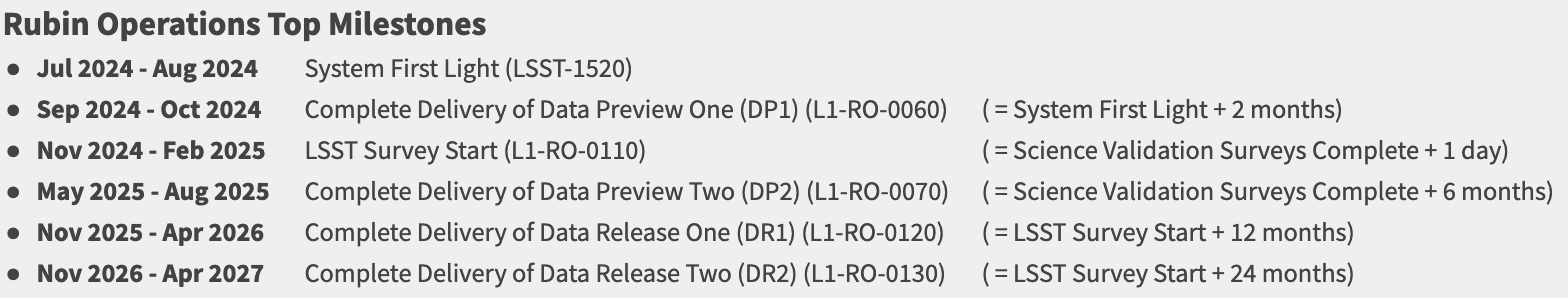
\includegraphics[width=\linewidth]{figures/DPR-milestones}
%\caption{Top milestones for the Early Science Program.}
%\label{tab:milestones}
%\end{table}

Milestone dates are given as min-max ranges to indicate the associated uncertainty. 
Typically the near date corresponds to the current Project forecast, plus any additional operational uncertainty.
The late date corresponds (approximately) to the current Project ``late date'' plus any additional operational uncertainty.
An intermediate (typically mid-range) date is used by the Rubin Operations teams for planning purposes. 

The LSST survey start is currently expected to be sometime between February 2025 and September 2025.
The timing of the Commissioning observations is somewhat less uncertain and the timing of the release of those data to the community can be projected to within a few months at the time of writing.

Table \ref{tab:timeline} shows the nominal date ranges for the various elements of the Early Science Program. 
The shaded region contains roughly 80\% of the probability, while the lefthand edge of the shaded range indicates the earliest date the milestone could be reached. 
The darker regions give a very rough indication of the +/-1 sigma error bars. 
Over the course of the commissioning period, we expect these shaded regions to shrink as our understanding of the remaining schedule uncertainty improves. 
However, there is still the possibility of the assumptions underlying these distributions being wrong: this is just our best estimate at the current time.

The next key milestone in the Early Science Program is the release of DP1
The late dates for the DP2 and DR1 milestones allow for the possibility that the Project completes within its late date, but in doing so spends less time on-sky with LSSTCam.
In this eventuality, the operations team would spend up to 2 months prior to commencing the 10-year LSST survey collecting more on-sky data to complement and extend the datasets collected during commissioning (see \S~\ref{ssec:scenarios}. 
\begin{table}[ht]
\centering
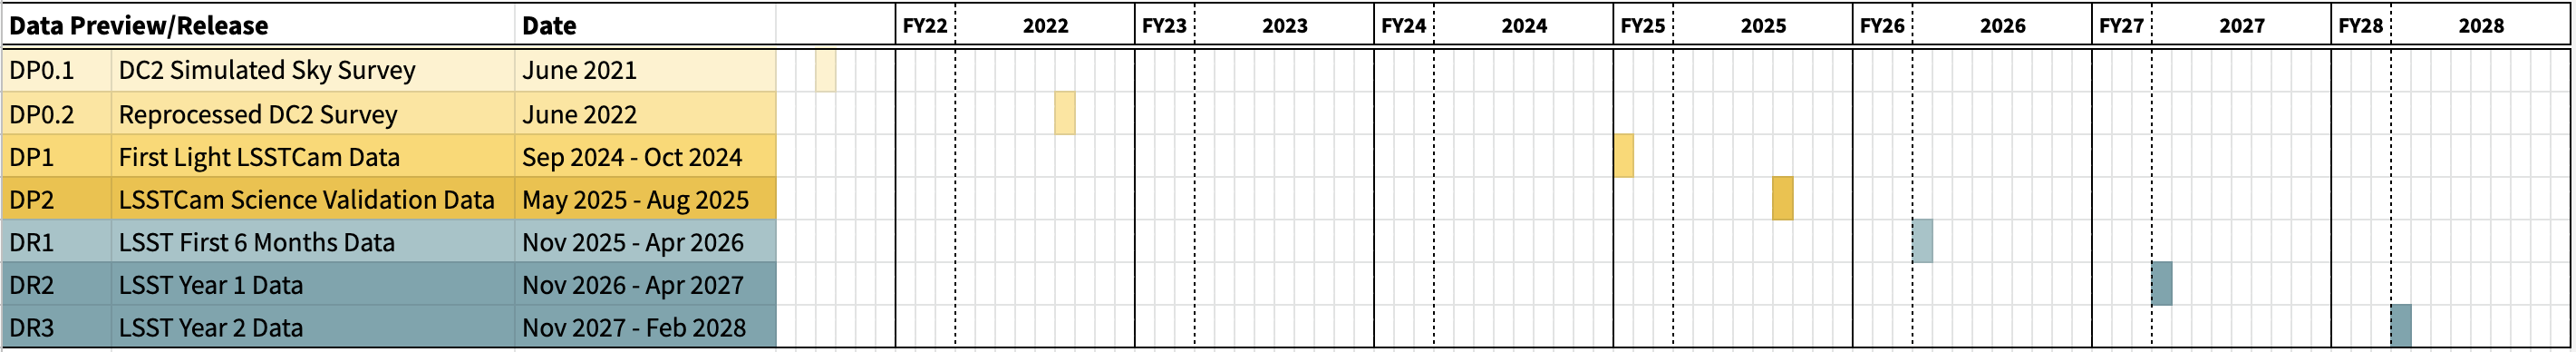
\includegraphics[width=\linewidth]{figures/DPR-timeline}
\caption{Nominal date ranges for the various elements of the Early Science Program.}
\label{tab:timeline}
\end{table}

Tables ~\ref{tab:milestones} and ~\ref{tab:timeline} will continue to be refined and updated in future version of this documents as the Early Science Program progresses.

\section{Science Drivers} \label{sec:science}

The various different science drivers outlined in \ref{sec:science} naturally lead to different priorities for template generations, e.g. solar system science prefers templates to be generated in the NES and Milky Way science would to would prefer templates for the galactic plane to optimise alert production in these areas in early operations. Other science will prefer templates in a number of filters to enable .. rather that larger area. 

\subsection{Time Domain}

The \tvssc reviewed the opportunities for \es for non time-critical and  time-critical science cases in \cite{Hambleton_2020} and \cite{Street_2020} respectively. 

\subsection{Solar System}

The \sssc reviewed opportunites for \es in \citeds{2020arXiv201005926L}. 
LSST is predicted to discover $\approx$ 6 million solar system planetesimals, providing in total over a billion photometric and astrometric measurements in 6 broad-band filters. 

\subsection{Static Science}
The baseline static science data sets will flow from \sv surveys carried out during commissioning. 

\subsection{Target of Opportunity}
Rubin Observatory will be prepared to take advantage of Targets of Opportunties (TOO) in the first year of operations (and hopefully SIT-COM). 

%% Leanne - restructure to present the prompt data products better 
% Add in from data preview section: 
%
%During routine LSST operations, prompt image data products will be made available 80 hours following camera readout.
%They include raw images, processed single visit images (PVIs), difference images, and template images.
%Access to unvetted PVIs and difference images in the first 6 months of the LSST is still to be decided.


\section{Alert Production in Commissioning and Early Operations}
\label{sec:pp}

\subsection{Processing Overview}

The \DPDD{} summarizes the pipelines which will be used during Prompt Processing to produce alerts as well as other prompt data products, including Solar System Processing.
In brief, raw images have instrument signatures removed and are photometrically and astrometrically calibrated.
When template images for the corresponding region of the sky are available, the template is subtracted from the new processed visit image and sources are detected on the image difference.
Alerts are then generated for all DIASources detected at five sigma in the difference.
At the end of the night, DIASources without a history of previous detection are input into Solar System Processing, which attempts to link them with other past detections and identify new Solar System objects.

Both Alert Production and Solar System Processing thus depend on the presence of template images.
During steady-state operations, these templates will be constructed during the annual Data Releases and will be built from the best available subset of images taken.
The input images for DRP-produced templates will accordingly have very good seeing and comprehensive spatial coverage.
All of these template characteristics help to ensure that image differencing is highly complete and highly pure.

To enable alert production to proceed during commissioning and early operations, it is necessary to accept templates of lower quality.
Because we have a smaller set of input images to choose from and uncertain knowledge about future observations, on-the-fly (or incremental) template generation necessarily must balance the trade off of earlier template availability against template quality and spatial completeness.
Substantial validation will be required to determine when to build incremental templates to maximize the net throughput of Early Science.
Nevertheless our goal is to enable Alert Generation to begin over at least a subset of the survey area as soon as the data are scientifically useful.

Coadding multiple images enables artifact rejection  \citeds{DMTN-080} and is formally required due to the noise-level requirements placed on the DM system. 
Additionally, the LSST survey is heavily dithered, so without coadding many images onto a common sky plane it is both difficult and inefficient to obtain image differences for a new pointing from past single images.
Finally, single-image templates do not permit removal of artifacts, transients, and moving objects from the template, creating additional false positive sources in the resulting differences.

Scientifically it is important that once a template is constructed for a given region of sky, it is used exclusively until it can be updated in the next Data Release.
Repeated changes to the template make it extremely difficult to construct usable lightcurves for objects from individual difference image sources: transient objects such as supernovae will be contaminated by changing flux levels from the evolving template, and variable objects such as variable stars and AGN will require repeated corrections for different template flux levels as well.

\subsection{Supporting Incremental Template Generation}

The Rubin Construction Data Management (DM) Science team (DM-SST) carried out a study of several options for Alert Production in Year 1, reported in \citeds{DMTN-107} : Options for Alert Production in LSST Operations Year 1.
Representatives of the Rubin Project Science Team (PST), DM-SST and Operations reviewed the proposed DM-SST options  and converged on a the following  strategy for Alerts in year 1:

\begin{itemize}
\item Commissioning Data Templates: Build templates, where possible, from all commissioning data before the start of year one, and use them to generate alerts during year one.
\item Year One Data Templates: Build templates progressively from data obtained during year one (e.g., on a monthly timescale), and use them to generate alerts during year one, either instead of, or in addition to using commissioning data to build templates.
\end{itemize}

To handle alert generation outside the template building process attached to the annual DRP, the Construction project initiated a change request to include incremental templates in the DM system workflow. This change has been accepted and is now part of the baselined DM project in construction. A summary of the changes is the following:

\begin{itemize}
\item LCR-2273: Construct Image Differencing Templates Outside DRP, new requirement 1.4.6 Template Coadds ID: DMS-REQ-0280, The DMS shall periodically create Template Images in each of the u,g,r,i,z,y passbands. Templates may be constructed as part of executing the Data Release Production payload, or by a separate execution of the Template Generation payload. Prior to their availability from Data Releases these coadds shall be created incrementally when sufficient data passing relevant quality criteria is available.
\item To enable artifact rejection, templates will be built with at least three images in year one, and five in subsequent years (Rubin OSS-REQ-0158). \footnote{The LSST SRD places well-defined criteria on the quality of the difference image and the amount of noise that a template can contribute to a difference image.These criteria result in a minimum of three images being needed to construct a template for use in year one, and five in subsequent years.}
\item Once a template is produced for a sky position and filter it will not be replaced until the next Data Release to avoid repeated baseline changes.
\item Templates are not necessarily built from the first N images that are collected.
\end{itemize}


\subsection{Alert Generation during Commissioning}

Due to the need to verify the instrument characteristics, template quality, and image differencing and Real/Bogus performance, real-time alerts will not be immediately available during the commissioning period.
However, the incremental template generation and alert production processes will be tested and optimized during commissioning with LSSTCam, resulting in a set of prompt data products, including alerts.
Broker teams will be given access to these alerts for development purposes as soon as they are produced to understand their characteristics and to help to validate their quality, rather than to enable rapid followup and Early Science.
The Alert and Prompt Product databases will be made available for query prior to the DP2 data release.

During commissioning templates will be generated incrementally over the maximal sky area supported by the available observations.
By the end of the commissioning period, coadd templates for use in difference imaging will only be available for $\approx$ 10\% of the sky.
Generating templates over a wide area is not an explicit goal of commissioning;  however, where possible, if commissioning observations are agnostic to pointing and filter, we would endeavour to choose a pointing and filter that maximizes building templates to enable early science.

Rubin aims to scale up alert production during commissioning with the aim of beginning routine Alert Production as soon as is feasible following System First light.
Once begun, Alert Production will then proceed continuously into the full LSST survey.
Alerts generated during commissioning may be produced with higher latency.
The commissioning period also provides an excellent opportunity to investigate how many visits in a given band are sufficient to construct a usable template.

Table~\ref{tab:prompt-data-products} lists the various alert and prompt processing data products currently planned at each phase of alert production during commissioning and the first two years of the LSST survey. 
Phase 1 covers the commissioning system optimization and science validation periods and phase 2 covers early survey operations.  

\begin{table}
\centering
\fontsize{6}{10}\selectfont 
\setlength{\tabcolsep}{6pt} % Default value: 6pt
{\renewcommand{\arraystretch}{1.3}
    \begin{tabular}{|p{0.31\linewidth} | p{0.32\linewidth}  | p{0.32\linewidth}|}
    \hline
    \multicolumn{3}{|l|}{{\fontsize{9}{12}\selectfont \color{RubinDarkTeal}\textbf{Rubin Early Science -- Alerts \& Prompt Products Scenario}}}  \\\hline\hline
  

\multirow{1}{*} {}  & 
        \tiny  \makecell{Phase 1: 3 -- 16 weeks post System First Light}  & 
        \tiny   \makecell{Phase 2: 18 -- 17 weeks post System First Light} \\[5pt] \cline{2-3}        
        {\parbox{0.5\linewidth}{\vspace{0.6cm} \textbf{Data Product}}}  &   
        { \makecell{ \textbf{LSSTCam Commissioning }  }}  & 
        {\makecell{\textbf{Year 1 Survey} \\ \textbf{Operations} }} 
         \\[10pt] \cline{2-3} \hline

\textbf{Alerts}     &  Alert volume and latency will improve throughout the commissioning period. Aiming for ``near-live'' brokered Alert stream by the end of LSSTCam Commissioning.  &  
Continued ramp up of the alert stream contingent on the availability of templates.  Alerts expected to reach near full volume and fidelity after DR1.  Alert stream latency in year 1 is 120 seconds. \\  \arrayrulecolor{gray}\hline
%
\textbf{PP Processed Visit Images}     & Commissioning of the PP image differencing and incremental template building. Prompt image release is embargoed during commissioning (\S~\ref{ssec:impact}).  &   Access to processed visit images as prompt products in the first 6 months of the LSST is TBD.      \\  \arrayrulecolor{gray}\hline
\textbf{PP Difference Images}     & Difference imaging will be somewhat limited, since the image template sky coverage will be sparse. Prompt image release is embargoed during commissioning (\S~\ref{ssec:impact}). &     Difference imaging will steadily increase as incremental template building increases the templates available. Access to PP difference images in the first 6 months of LSST is TBD.    \\\hline
%
\textbf{PP Catalogs}    &   Queryable PPDB available at shared risk. &  PPDB available for query. \\ 
 (DIASources, DIAObjects, DIAForcedSources)  & & \\\hline
%
\textbf{PP SSP Catalogs}   &   Measurements of known SSObjects sent to the MPC whenever difference images are available. Searches for new SSObjects performed if appropriately-cadenced data is present. SSP Catalogs likely unavailable for query in the PPDB. &   Standard SSP Daily Data Products produced from difference images as they are available and reported to the MPC. SSP catalogs available for query in the PPDB.  \\  \hline

\arrayrulecolor{black}\hline
\end{tabular}}
\caption{Summary of Prompt data products expected during commissioning and year 1 of survey observations..}
\label{tab:prompt-data-products}
\end{table}

%\begin{table}[ht]
%\centering
%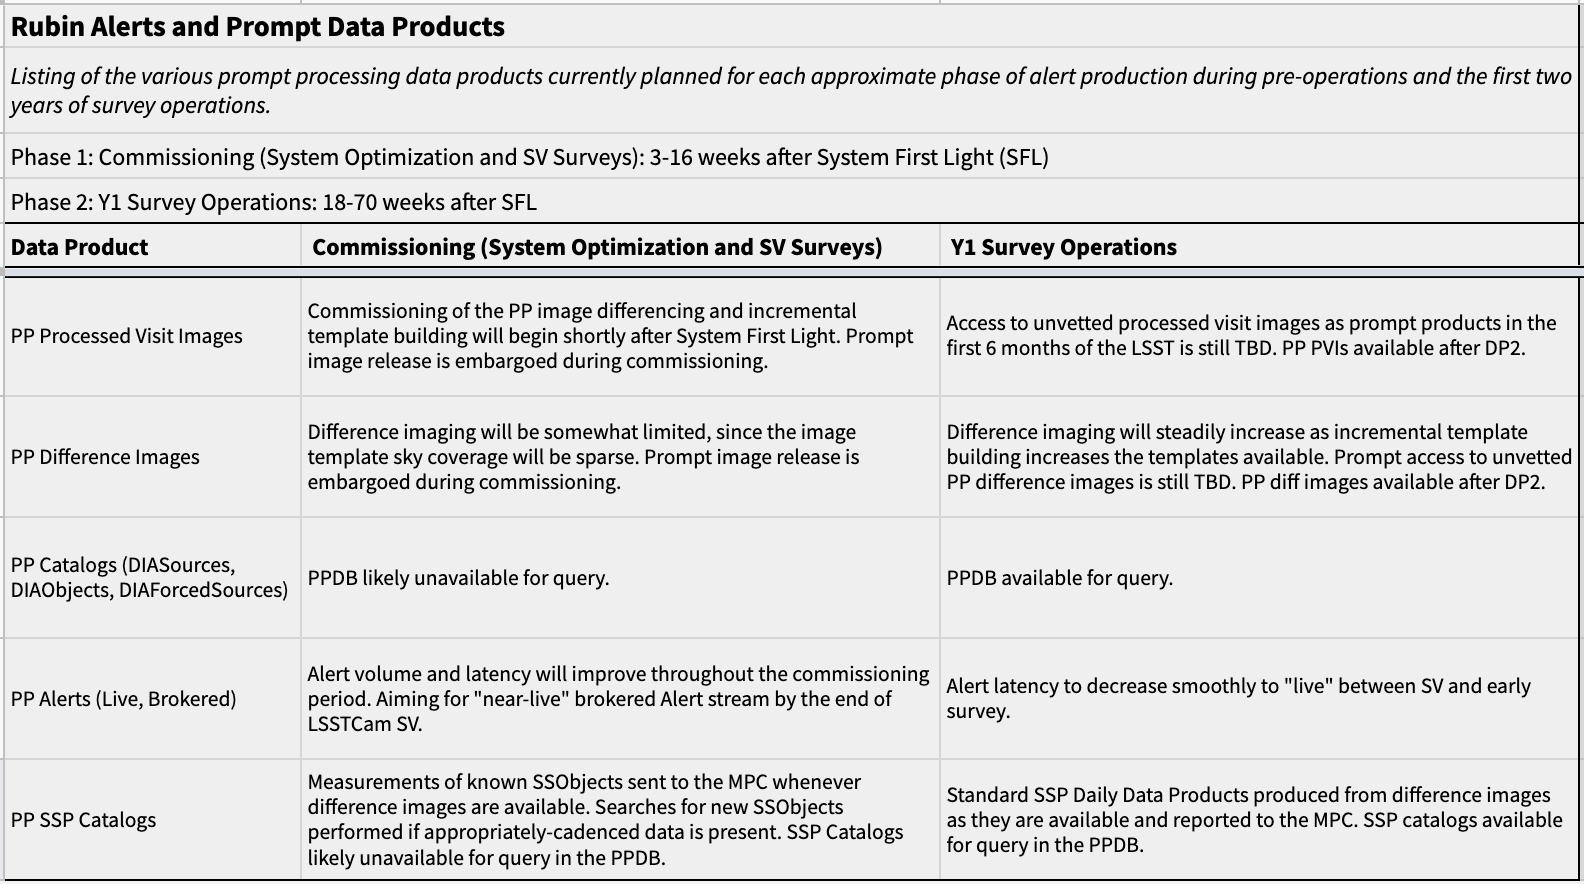
\includegraphics[width=0.9\linewidth]{figures/Prompt-products}
%\caption{Summary of prompt data products expected during commissioning and year 1 survey observations.}
%\label{tab:prompt-data-products}
%\end{table}

\section{Rubin Observatory Commissioning}
\label{sec:commissioning}

\subsection{Commissioning Schedule}
\label{ssec:commissioning-schedule}

Following the October 2023 project schedule workshop, the Rubin Construction Project is re-optimizing the sequence of integration activities in light of recent subcomponent delays, in particular, (i) delay in shipment of the Camera and (ii) necessary repairs to the  summit dome crane.
If current estimates hold, it will be beneficial to re-implement on-sky data-taking with ComCam (previously removed from the schedule in order to install LSSTCam sooner).
The updated plan calls for on-sky data to be taken with ComCam for approximately two months, around July-August 2024 to support Telescope commissioning, primarily the Active Optics System. 
This is approximately four months earlier than could be done with LSSTCam. 

\begin{figure}[htb]
\centering
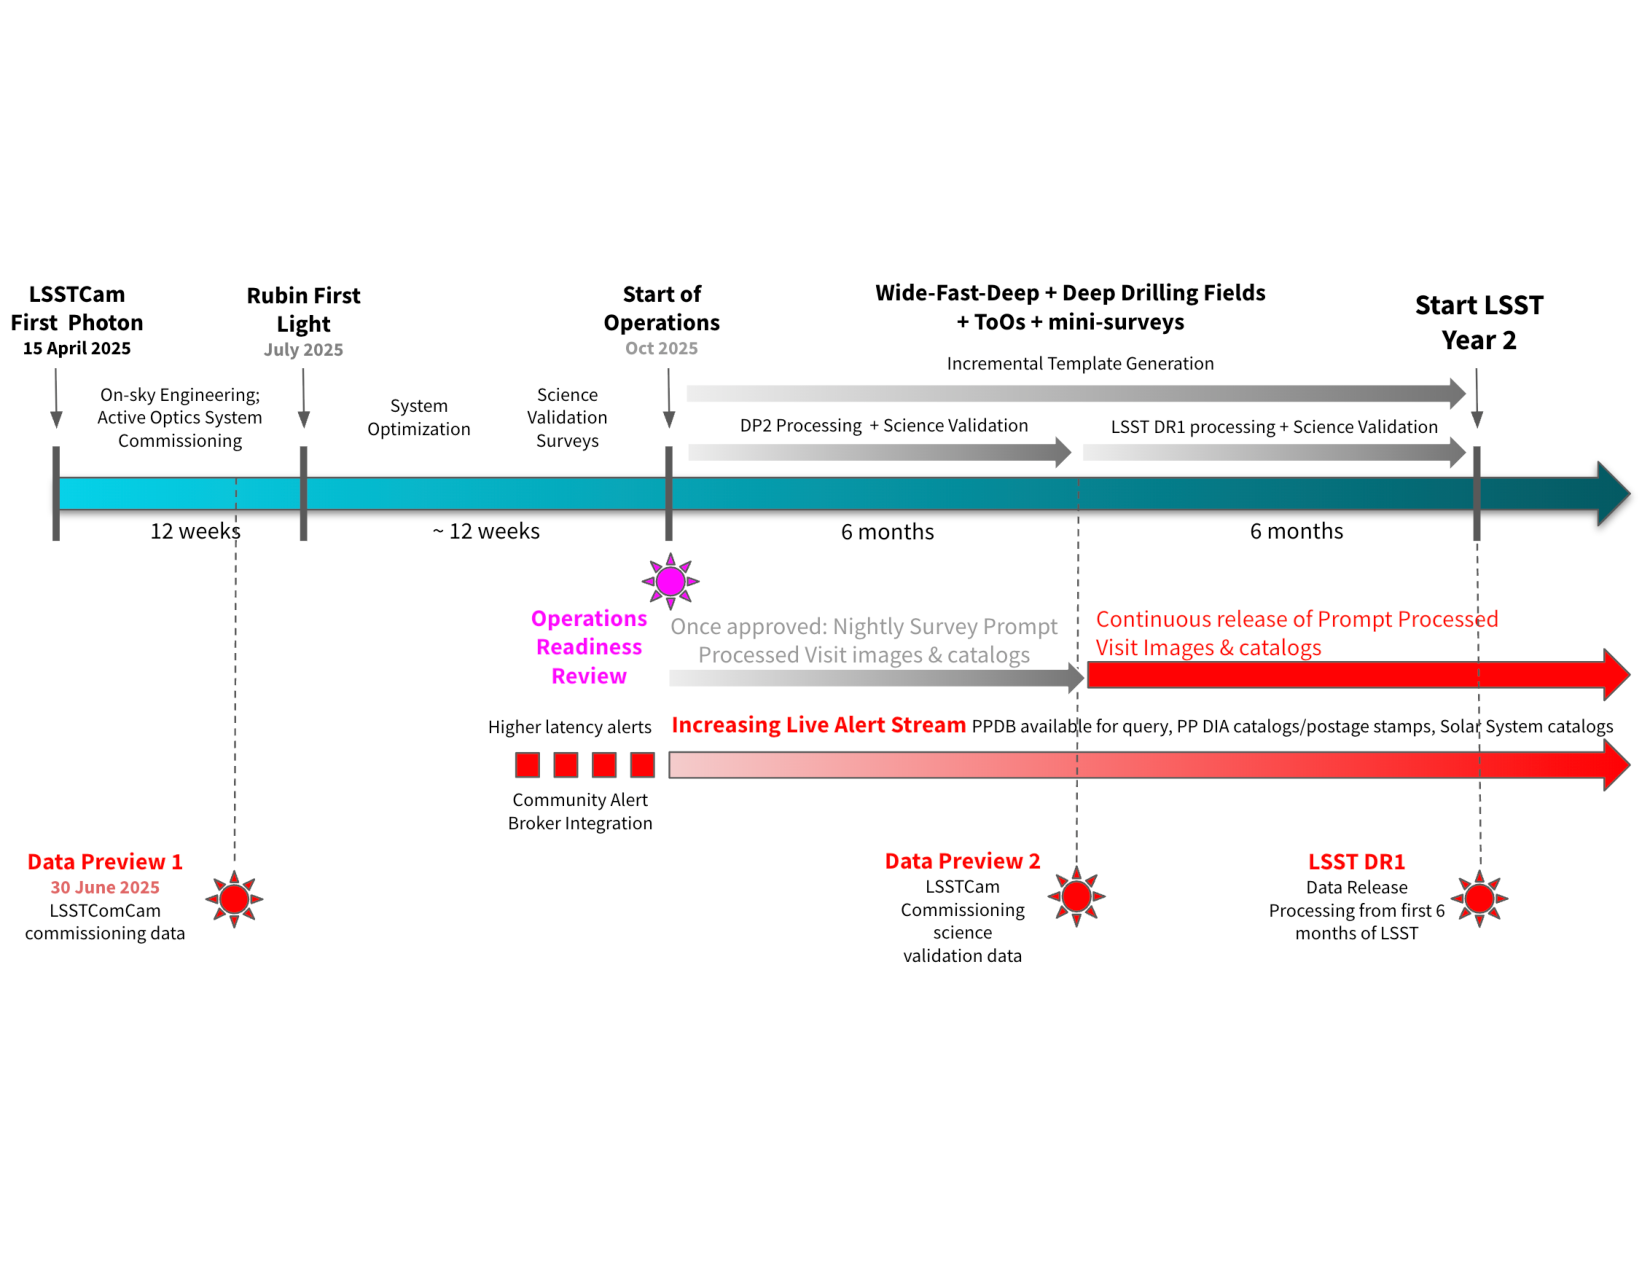
\includegraphics[width=0.98\linewidth]{figures/rubinobs_on-sky_commissioning_and_early_science.pdf}
\caption{Detailed schedule of commissioning  and early science activities relative to System First Light, as of October 2023.}
\label{fig:commissioning-es-schedule}
\vspace{0.1cm}
\end{figure}

Figure~\ref{fig:commissioning-es-schedule} shows the detailed schedule of commissioning and early science activities relative to System First Light, as of October 2023.
System First Light is currently expected in January 2025 (\S~\ref{sec:timeline}), about 7 weeks after LSSTCam First Photon.
The total amount of science validation time currently planned is about 8 weeks.  
LSST data taking is expected to start 4-10 months after System First Light depending on construction schedule uncertainty and Operations readiness to start the survey following the start of full Survey Operations.

The project schedule will continue to evolve as the remaining subcomponents are delivered. 
The final decision concerning ComCam on-sky data taking will be taken in February 2024.

\subsection{Commissioning Milestones}
\label{ssec:commissioning-milestones}

Commissioning work is being planned around three major milestones, \textit{ComCam First Photon}, \textit{LSSTCam First Photon} and \textit{System First Light}. 

\textbf{ComCam First Photon}: The first image of the night sky produced by photons passing through the Rubin optical system and detected by the Commissioning Camera (ComCam).

\textbf {LSSTCam First Photon}: The first image of the night sky produced by photons passing through the Rubin optical system and detected by the LSST Science Camera (LSSTCam).

\textbf {System First Light}: Defined as the point at which we can routinely acquire science-grade imaging across the LSSTCam full focal plane and have a well understood technical path towards meeting the Construction Completeness criteria   \citeds{sitcomtn-061}.
Also referred to as \textbf{First Light}. 

As the Project continues to optimize the sequence of integration activities and if it becomes no longer beneficial to go on-sky with ComCam, the ComCam First Photon milestone will be descoped. 
LSSTCam First Photon occurs following the successful completion of system integration. 
There are no quality criteria applied to achieving  neither the ComCam nor LSSTCam First Photon milestones. 
System First Light  marks the end of the  on-sky engineering phase and the start of the System Optimization and Science Validation phases of commissioning.
During the period between ComCam First Photon and System First Light will focus on fine tuning the system including optical alignment and improving the image quality, collecting calibration data, and carrying out \textit{First Look} science programs. 

For a detailed description of all the commissioning milestones and the most current dates, see \citeds{dmtn-232}.


\subsection{Commissioning Observations}
\label{ssec:commissioning-observations}

Figure~\ref{fig:commissioning} shows the high level plan for the Rubin commissioning observations. 
Commissioning data collection is planned to take place in phases.
The \textit{On-Sky Engineering} phase may be carried out with either ComCam and/or LSSTCam, depending on future re-optimization of the sequence of integration activities (\S~\ref{ssec:commissioning-schedule})
During the \textit{System Optimization} phase,  a set of observations designed to help optimize the system will be taken during the System Optimization phase before the Science Validation Surveys are carried out. 
The SV Surveys are designed to support scientific analyses that validate the system's performance, and allow Rubin to demonstrate operations readiness \citeds{SITCOMTN-005}.

\begin{figure}[htb]
\centering
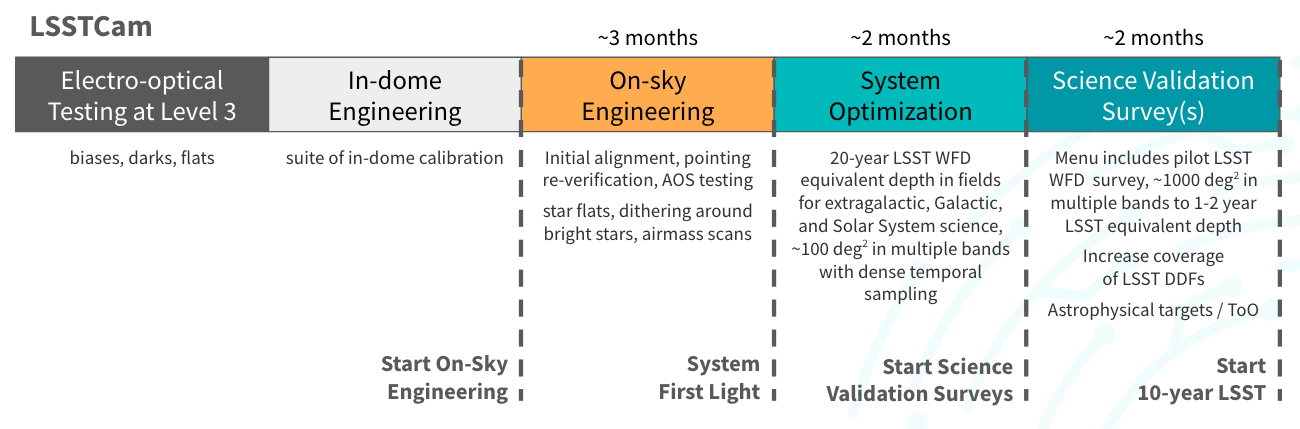
\includegraphics[width=0.95\linewidth]{figures/commissioning-plan}
\caption{Outline plan for the collection of commissioning data, as of October 2023.}
\label{fig:commissioning}
\end{figure}

Figure~\ref{fig:commissioning} also indicates a number of planned key components of the System Optimization and SV phases.
These include a LSST wide-fast-deep (WFD) 1-2 year equivalent depth ``pilot'' survey.
Field selection will be carried out by the Commissioning Team, taking into account a wide variety of constraints as well as a ``menu'' of science opportunities to which the LSST Science Community has contributed.
Details of the plans for commissioning observations will be made available as those plans converge, in this technote and other documents as cited.
% Early Science Data Products
% Responsible: Leanne Guy
\section{Early Science Data Products}
\label{sec:data}

Here we provide a summary of the data products that are expected to be made available as part of the \esp.
The definitive source for all LSST data products is the Data Products Definition Document (DPDD), \citep{LSE-163}.
However, each pre-operations data preview and survey data release will be accompanied by its own DPDD, giving e.g. the catalog database schema for the tables included in that dataset.
For an introduction to the Rubin data products, see \citet{RubinDataProductsAbridged}.
For an example data release DPDD, see the online DP0.2 documentation.\footnote{\url{https://dp0-2.lsst.io/data-products-dp0-2/}}
The Rubin data rights policy is described in  \cite{RDO-013}.

\subsection{Prompt data products}

Prompt data products are described in detail in the Data Products Definition Document (\DPDD).
Alert packets are triggered by difference image source detections and transmitted to community alert brokers\footnote{See \url{https://www.lsst.org/scientists/alert-brokers} for the list of selected brokers.} and are publicly available.
Similarly, daily Solar System Processing identifies new Solar System Objects from difference image sources and reports those publicly to the Minor Planet Center.

Catalog data products, as well as services for running user-generated processing on the data, are available to Rubin Data Rights holders after 24 hours through the Rubin Science Platform (\S~\ref{ssec:dataaccess}).
\DIASource, \DIAObject, and \SSObject catalogs are queryable using VO interfaces to the Prompt Products Database.
Image products are available after 80 hours.

\subsection{Data Release data products}
Static science datasets for Early Science will flow from the \svs in commissioning.
Images and catalogs from the DRP of the commissioning data will be made available to data rights holders in the form of Data Previews via the access mechanisms described in \S~\ref{ssec:dataaccess}.
Due to the relatively short time periods available for commissioning observations (\S~\ref{ssec:scenarios}), these Data Previews will necessarily be limited in their area and temporal coverage relative to full Data Releases, however all Data Preview data products will be in the same science data model format as for future Data Releases.

\subsection{Access to \es data products}\label{ssec:dataaccess}
Alerts will be accessible by the community via one or more of the nine Rubin-endorsed Community Brokers.
The Rubin Data Rights community will access the Rubin data products via the Rubin Science Platform, \citep{LSE-319}.

\subsection{Summary of expected \es data products}

The tables in this section outline which data products can be expected in each \es data preview and data release, and when.

\begin{table}
\caption{Summary of data products expected in each data preview and early survey data release, as of October 2022.}
\label{tab:summary}
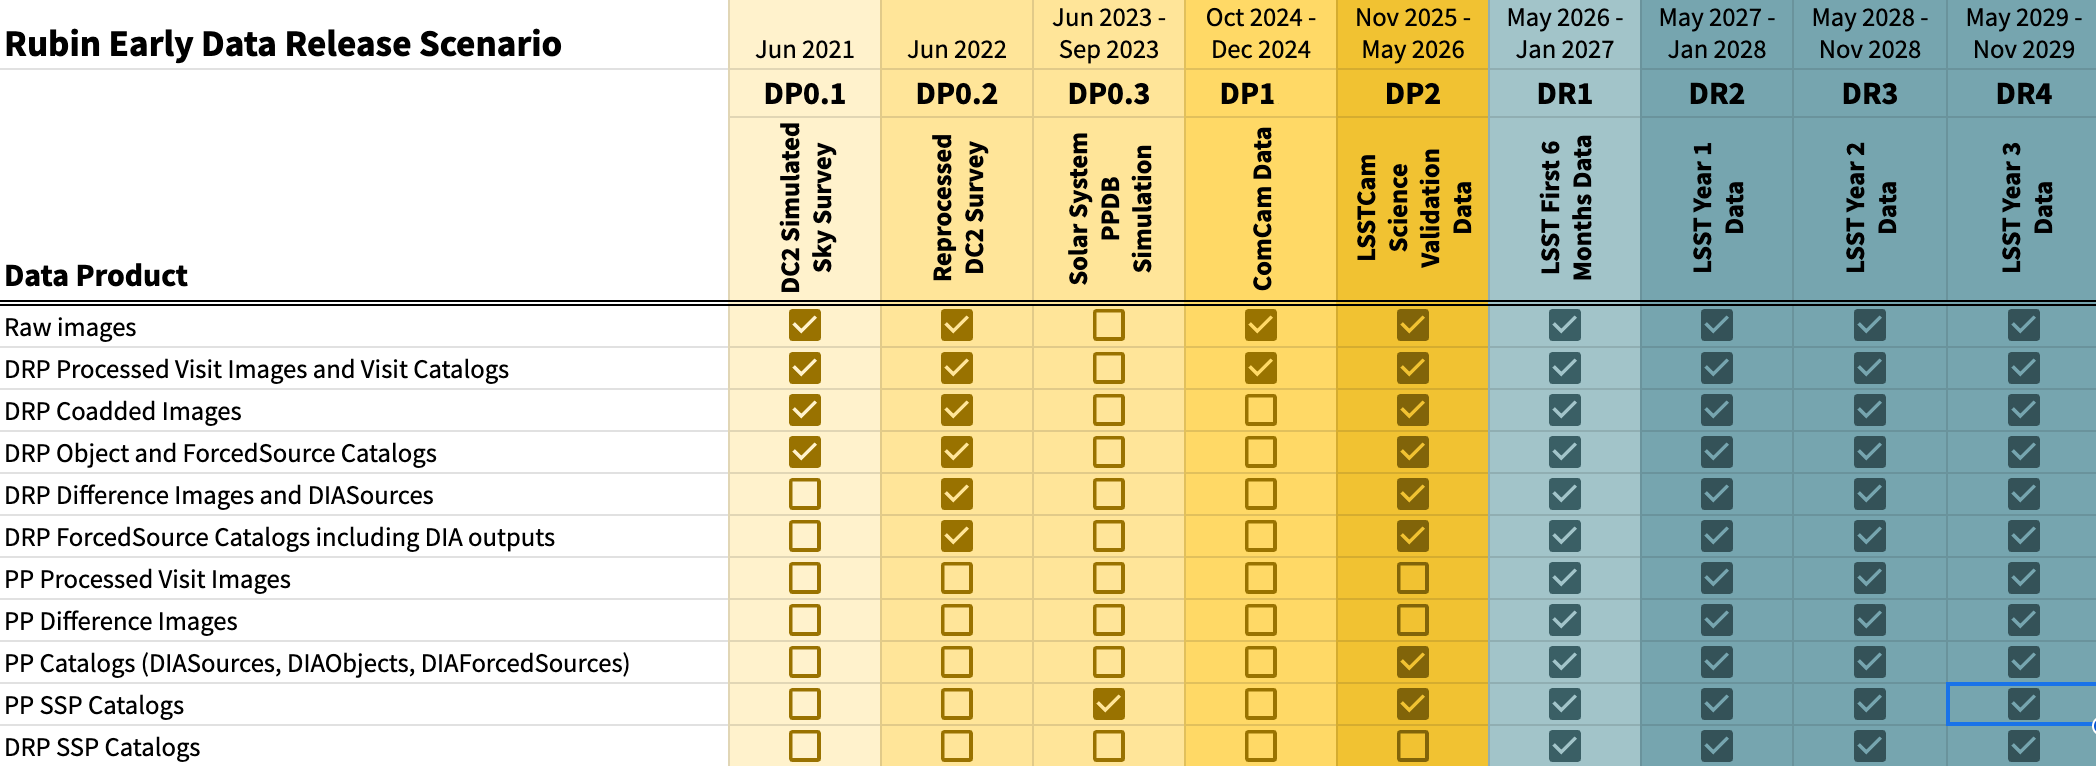
\includegraphics[width=\linewidth]{figures/DPR-summary}
\end{table}

\begin{table}
\caption{Summary of data products expected in DP1, as of October 2022.}
\label{tab:dp-one-products}
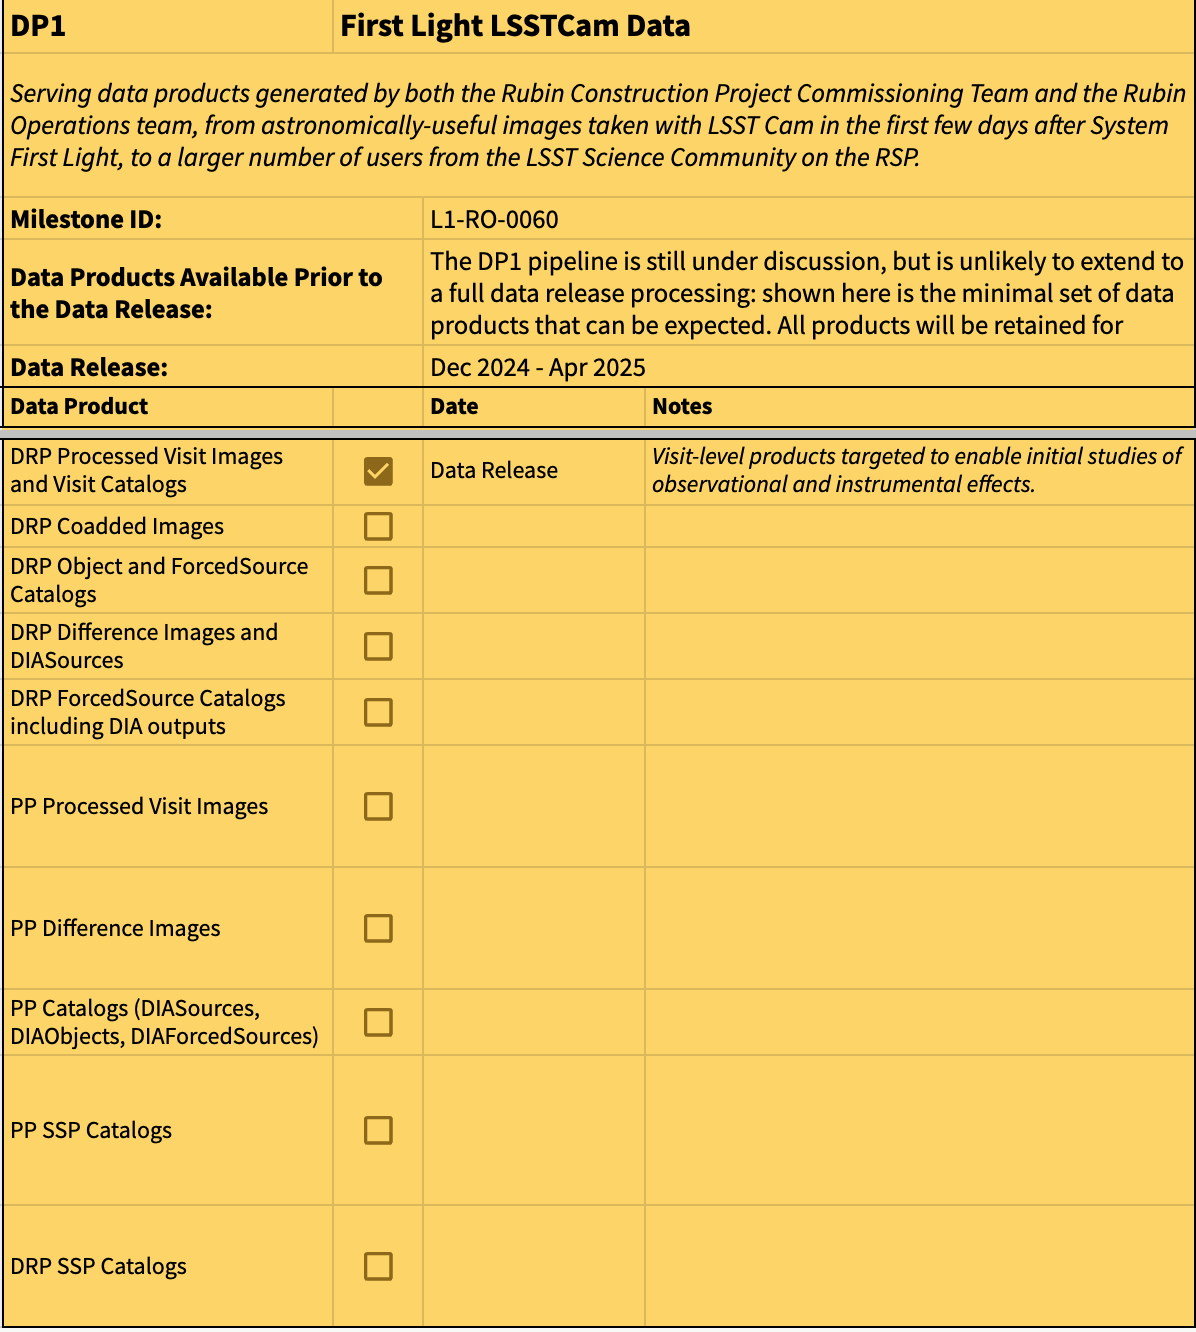
\includegraphics[width=\linewidth]{figures/DP1-products}
\end{table}

\begin{table}
\caption{Summary of data products expected in DP2, as of October 2022.}
\label{tab:dp-two-products}
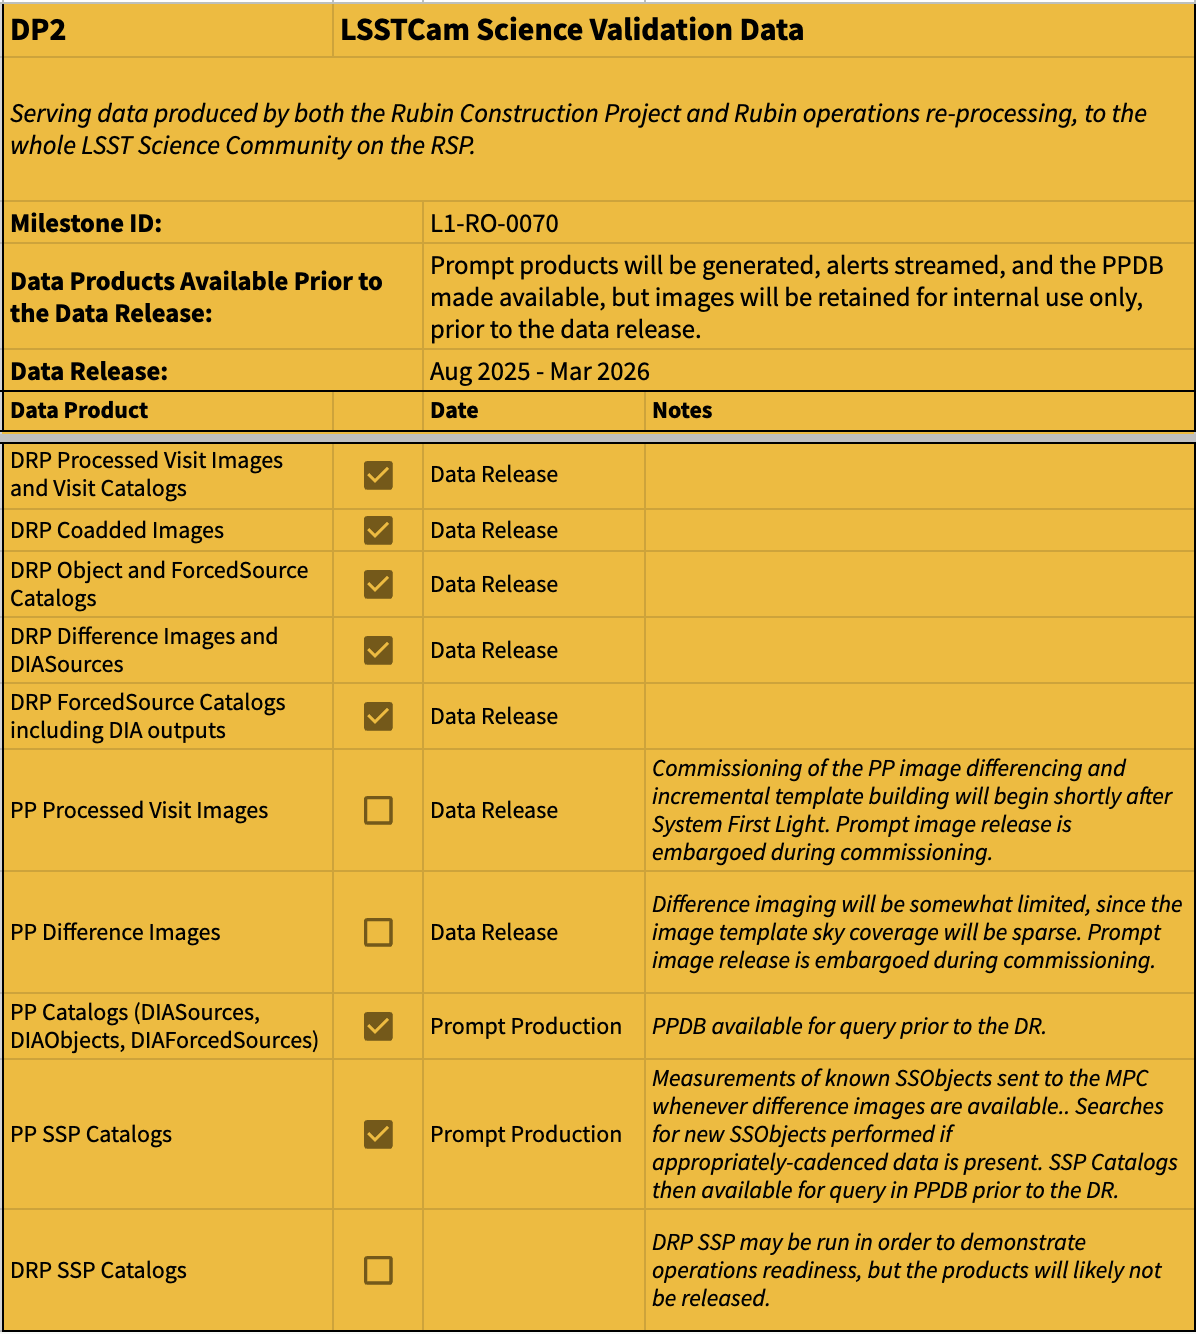
\includegraphics[width=\linewidth]{figures/DP2-products}
\end{table}

\begin{table}
\caption{Summary of data products expected in DR1, as of October 2022.}
\label{tab:dr-one-products}
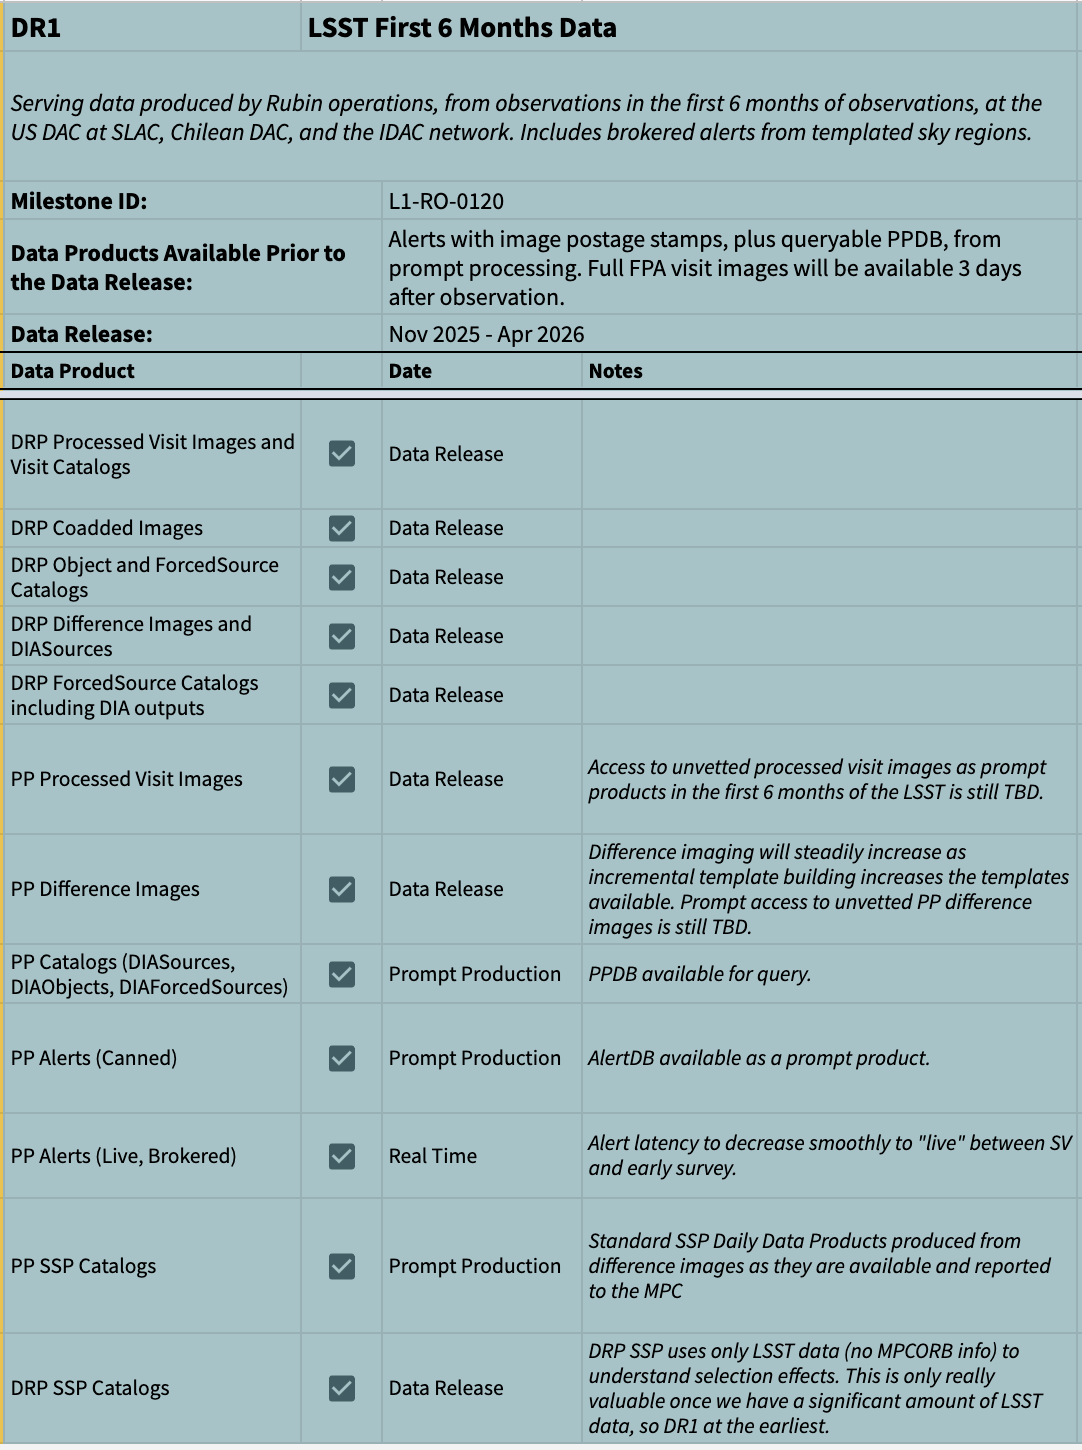
\includegraphics[width=\linewidth]{figures/DR1-products}
\end{table}

% Implication of early science on the full survey cadence
% Responsible : Zeljko
\section{Survey Cadence}

Early Science observations must align with main survey and ultimate long-term science goals. 
Details on the implications for the Survey Cadence of the \esp will be added in future as the outcome of commissioning becomes clear.  


\section{Community Engagement}

Rubin Observatory will work closely with the community on the detailed design of the \esp. 

\subsection{Survey Cadence Optimization Committee}
The \href{https://www.lsst.org/content/charge-survey-cadence-optimization-committee-scoc}{Survey Cadence Optimization Committee (SCOC)} is an advisory committee to the Rubin Observatory Operations Director consisting of 10 members from drawn almost entirely from the science community.
It began in 2020 and will be a standing committee throughout the life of Rubin Observatory operations. 

Early Science observations must align with main survey and ultimate long-term science goals; the SCOC will be involved in all aspects of development of the \esp. 
Specifically, the SCOC will make specific recommendations for Early Science observations, based on the plans for commissioning and the realized performance of the telescope and software. 


\subsection{Community Forum}

The Rubin Observatory Community Platform has a \href{https://community.lsst.org/t/about-the-early-science-category/5775}{dedicated category for Early Science}, where  community members can open discussions on the topic of early science. 

\subsection{Community Input}

A process will be put in place to formally solicit input from the community. 
Several science collaborations have already been pro-active in providing input on considerations for template generation in year one on both the community forum and as research notes. 

\appendix
% Include all the relevant bib files.
% https://lsst-texmf.lsst.io/lsstdoc.html#bibliographies
\section{References} \label{sec:bib}
\renewcommand{\refname}{} % Suppress default Bibliography section
\bibliography{local,lsst,lsst-dm,refs_ads,refs,books}

% Make sure lsst-texmf/bin/generateAcronyms.py is in your path
\section{Acronyms} \label{sec:acronyms}
\addtocounter{table}{-1}
\begin{longtable}{p{0.145\textwidth}p{0.8\textwidth}}\hline
\textbf{Acronym} & \textbf{Description}  \\\hline

 &  \\\hline
B & Byte (8 bit) \\\hline
DM & Data Management \\\hline
DM-SST & DM System Science Team \\\hline
DMS & Data Management Subsystem \\\hline
DMS-REQ & Data Management System Requirements prefix \\\hline
DMTN & DM Technical Note \\\hline
DR1 & Data Release 1 \\\hline
DRP & Data Release Processing \\\hline
LCR & LSST Change Request \\\hline
LSST & Legacy Survey of Space and Time (formerly Large Synoptic Survey Telescope) \\\hline
MAF & Metrics Ananlysis Framework \\\hline
OSS & Observatory System Specifications; LSE-30 \\\hline
PP & Prompt Processing \\\hline
PST & Project Science Team \\\hline
RTN & Rubin Technical Note \\\hline
SIT & System Integration, Test \\\hline
SIT-COM & System Integration, Test, and Commissioning \\\hline
SST & Subsystem Science Team \\\hline
SV & Science Verification \\\hline
TOO & Target Of Opportunity \\\hline
\end{longtable}

% If you want glossary uncomment below -- comment out the two lines above
%\printglossaries

\end{document}
